\mychapter{state-of-the-art}{State of the Art in Provisioning}

There already exists scientific research projects, \myac{API}s, frameworks 
and other technologies which aim at consolidating, interfacing and utilizing cloud technologies.
This chapter introduces some of these concepts, and does this by dividing the chapter into four parts:
\begin{enumerate}
  \item Model-Driven Approaches which aims presenting frameworks and projects that utilize
  models on a larger scale.
  \item \myac{API}s are about frameworks that connects to cloud providers, often with multicloud support,
  these projects can be used as middleware for other systems.
  \item Deployments are about projects that do full deployment of applications, inclusing provisioning.
  These are often more academic.
  Lastly the chapter will discuss \iitem Example of cloud surveys, some real-world examples
  that might not be directly related to provisioning but are important and interesting regardless.
\end{enumerate}

\section{Model-Driven Approaches}

\paragraph{Amazon AWS CloudFormation.}~\cite{aws}

\begin{figure}[tb]
  \begin{center}
    \begin{minted}[mathescape,
                   linenos,
                   numbersep=5pt,
                   frame=lines,
                   framesep=2mm]{json}
{
  "Description": "Create an EC2 instance",
  "Parameters": {
    "KeyPair": {
      "Description": "For SSH access",
      "Type": "String"
    }
  },
  "Resources": {
    "Ec2Instance": {
      "Type": "AWS::EC2::Instance",
      "Properties": {
        "KeyName": { "Ref": "KeyPair" },
        "ImageId": "ami-1234abcd" 
      }
    }
  },
  "Outputs" : {
    "InstanceId": {
     "Description": "Instace ID of created instance",
     "Value": { "Ref": "Ec2Instance" }
    }
  },
  "AWSTemplateFormatVersion": "2010-09-09"
}
    \end{minted}
  \end{center}
  \caption{AWS CloudFormation template.}
  \label{fig:cloudformation-template}
\end{figure}



This is a service provided by Amazon from their popular \myac{AWS}.
It give users the ability to create template files in form of 
\myac{JSON} as seen in ~\citefig{cloudformation-template}, 
which they can load into \myac{AWS} to create stacks of resources. 
A \emph{stack} is a defined set of resources in different amount and sizes, 
such as numerous instances,
one or more databases and a load balancer, although what types and sizes of resources is ambiguous.
To provision a stack with CloudFormation the template file (in \myac{JSON} format) is first uploaded to
\myac{AWS} which makes it accessible from \myac{AWS} Management Console.

The template consist of three main sections, 
\begin{ii}
  \iitem \emph{Parameters}, 
  \iitem \emph{Resources} and 
  \iitem \emph{Outputs}.
\end{ii}
The \emph{Parameters} section makes it possible to send parameters into the template, 
with this the template becomes a macro language by replacing 
references in the \emph{Resources} section with inputs from users. 
Input to the parameters are given inside the management console when 
provisioning a stack with a given template.
The \emph{Resource} section define types of resources that should be provisioned, the \emph{Type}
property is based on a set of predefined resource types such as \emph{AWS::EC2::Instance}
in Java package style.
The last section, \emph{Output}, will generate output to users when provisioning is complete,
here it is possible for users to pick from a set of variables to get the information they need.

This template system makes it easier for users to duplicate a setup many times, 
and as the templates support parameters this process can be as dynamic as the user design it to be. 
This is a model in form or lexical syntax, both the template itself 
and the resources that can be used.
For a company that is fresh in the world of cloud computing this service 
could be considered too advance. 
This is mainly meant for users that want to replicate a certain stack, 
with the ability to provide custom parameters. 
Once a stack is deployed it is only maintainable through the \myac{AWS} Management Console, 
and not through template files. 
The format that Amazon uses for the templates is a good format, 
the syntax is in form of \myac{JSON} which is readable and easy to use, 
but the structure and semantics of the template itself is not used by any 
other providers or cloud management tooling, 
so it can not be considered a multicloud solution. 
Even though \myac{JSON} is a readable format, 
it does not make it viable as a presentation medium on a business level.

\paragraph{CA Applogic.}~\cite{applogic}

\begin{figure}
  \begin{center}
  \end{center}
  \caption{CA Applogic}
    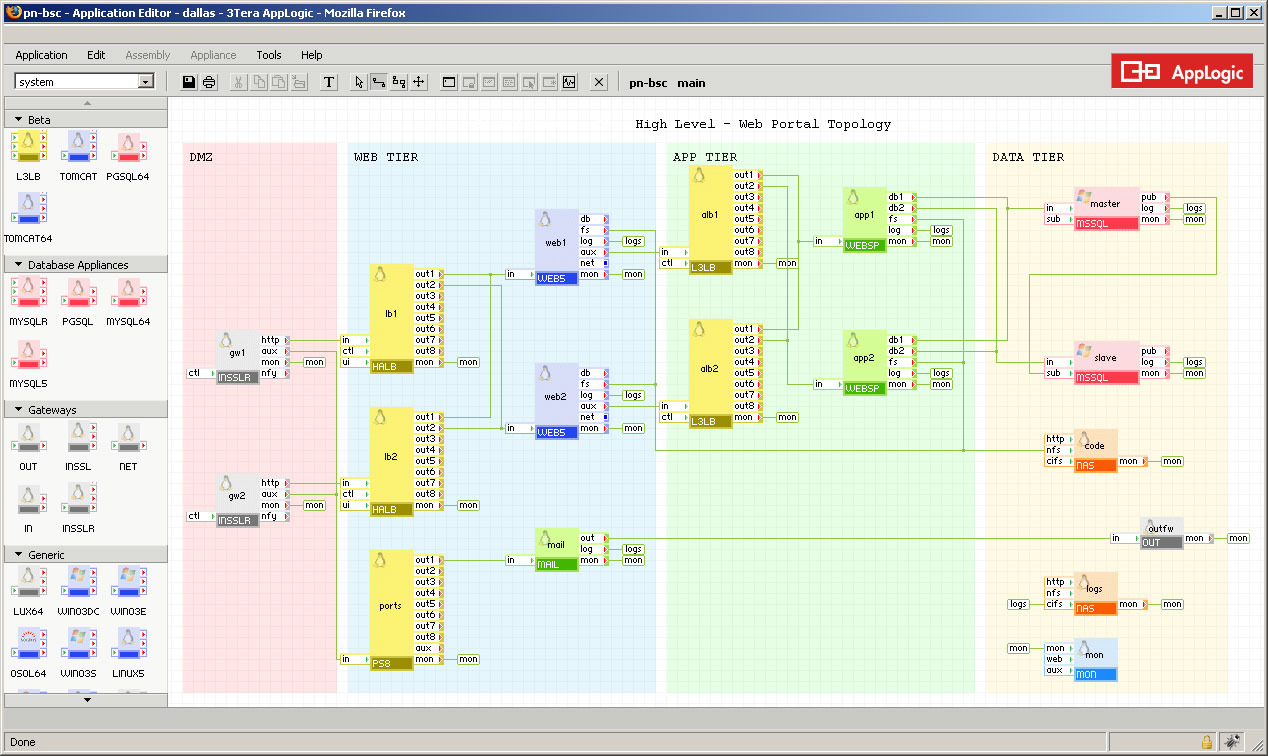
\includegraphics[width=\linewidth]{img/applogic.jpg}
  \label{fig:applogic}
\end{figure}


The Applogic platform is designed to manage CAs private cloud 
infrastructure~\cite{introducing-cloud-services}.
It also has a web based interface which let users manage their cloud resources 
as shown in~\citefig{applogic} which use and benefit from a model based approach.
It is based on graphical models which support interactive ``drag and drop'' functionalities.
This interface let users configure their deployments through a diagram with familiarities to 
\myac{UML} component diagrams with interfaces and assembly connectors. 
They let users configure a selection of third party applications, 
such as Apache and MySQL, as well as network security, instances and monitoring. 
What CA has created is both an easy way into the cloud and it utilizes 
the advantages of model realizations. 
Their solution will also prove beneficial when conducting business level consulting
as it visualizes the structural layout of an application.
But this solution is only made for private clouds running their own controller, 
this can prove troublesome for migration, both in to and out of the infrastructure.

\paragraph{Madeira Cloud.}~\cite{madeiracloud}

\begin{figure}[tb]
  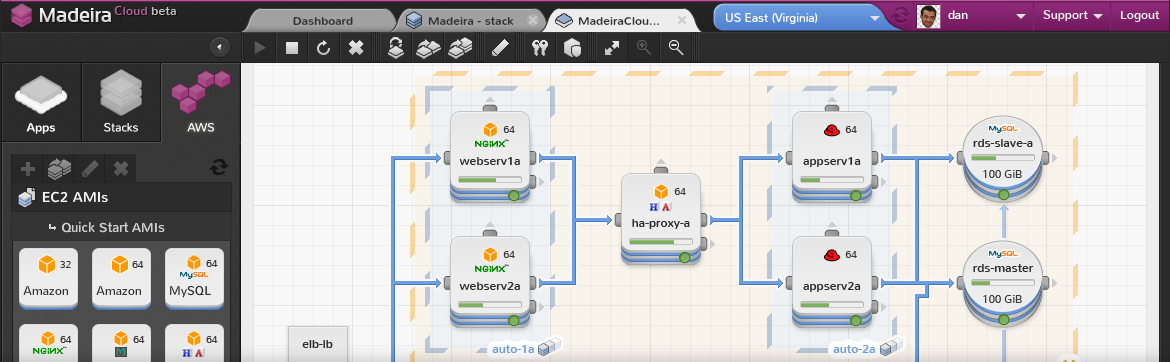
\includegraphics[width=\linewidth]{img/madeira.png}
  \caption{Madeira Cloud screenshot.}
  \label{fig:madiera}
\end{figure}


Madeira have created a tool which is similar to CA Applogic, but instead of focusing
on a private cloud solution they have created a tool specifically for \myac{AWS} \myac{EC2}.
Users can create \emph{stacks} with the available services in \myac{AWS} through 
dynamic diagrams.
Like CA Applogic their tool is also proprietary, but on the other hand they support
a free account which can be used to test their service out.
One would also need a \myac{AWS} account as an addition.

These \emph{stacks} are live representations of the architecture and can be found 
and managed in the \myac{AWS} console as other \myac{AWS} services.
They also support storing running systems into template files which can be used
to redeploy identical copies and it should also handle configuration conflicts.
For identifying servers they use hostnames, which are bound to specific instances 
so end users don't have to bother with IP addresses.

\mysection{API}{APIs}

Extensive work have been done towards simplifying and combining cloud technologies through
abstractions, interfaces and integrations.
Much of this work is in form of \myac{API}s, mostly in two different forms.
Either as programming libraries that can be utilized directly from a given 
programming language or environment such as Java or Python.
The other common solution is to have an online facade against public providers,
in this solution the APIs are mostly in \myac{REST} form.
\myac{REST}~\cite{rest:fielding00} is a software architecture for management of web resources
on a service. It uses the \myac{HTTP} and consecutive methods such as GET, POST, PUT and DELETE
to do tasks such as retrieve lists, items and create items.
\myac{API}s can be considered modeling approaches based on the fact they have a topology 
and hierarchical structure, 
but it is not a distinct modeling. 
A modeling language could overlay the code and help providing a clear overview, 
but the language directly would not provide a good overview of deployment. 
And links between resources can be hard to see, 
as the \myac{API} lacks correlation between resources and method calls. 

\begin{figure}[tb]

  \begin{tikzpicture}[scale=1, transform shape]
    \node (Framework) [box, minimum width=8cm, minimum height=5cm] { };

    \node (Interface) [class, text width=2cm, yshift=0.25cm, xshift=-2.5cm] { 
      \textbf{Common  \\ interface} 
    };

    \node (Driver-EC2) [class, right=of Interface] { 
      \textbf{Driver - EC2} 
    };
    \node (Driver-Rackspace) [class, above=of Driver-EC2] { 
      \textbf{Driver - Rackspace} 
    };
    \node (Driver-Azure) [class, below=of Driver-EC2] { 
      \textbf{Driver - Azure} 
    };

    \node (EC2) [tcloud, xshift=1cm, right=of Driver-EC2] { \textbf{EC2} };
    \node (Rackspace) [tcloud, xshift=1cm, right=of Driver-Rackspace] { \textbf{Rackspace} };
    \node (Azure) [tcloud, xshift=1cm, right=of Driver-Azure] { \textbf{Azure} };

    \draw[arrow] (Interface) -- (Driver-EC2.west);
    \draw[arrow] (Interface) -- (Driver-Rackspace.west);
    \draw[arrow] (Interface) -- (Driver-Azure.west);

    \draw[arrow] (Driver-EC2) -- (EC2);
    \draw[arrow] (Driver-Rackspace) -- (Rackspace);
    \draw[arrow] (Driver-Azure) -- (Azure);
  \end{tikzpicture}

  \caption{Cloud drivers.}
  \label{fig:drivers}
\end{figure}


\infobox{
  \subparagraph{Driver.}
  All the \myac{API} solutions use the term ``\emph{driver}'', it represents
  a module or component that fit into existing software and extend the support
  of external connections without changing the interface.
  A cloud \emph{driver} connects a given software to an existing cloud provider
  through this providers web based \myac{API} (\myac{REST}), illustrated in \citefig{drivers}.
}

\paragraph{jclouds.}~\cite{jclouds}

This is a library written in Java and can be used from any \myac{JVM}-based language.
Provider support is implemented in \emph{drivers}, and they even support deployments
to some \myac{PaaS} solutions such as \myac{GAE}.
\emph{jclouds} divide their library in two different parts, one for computing powers 
such as \myac{EC2} and one for \emph{blob} storage like S3. 
Some blob storage services are accessible on the compute side of the library such
as \myac{EBS}.
They support ``dry runs'' so a stack can be deployed as a simulation, not 
actually deploying it to a public cloud.
This is beneficial for testing deployments, and writing unit tests without initializing
connections, the library enhance this by providing a stub aimed at testing.

\paragraph{libcloud.}~\cite{libcloud}

Libcloud is an \myac{API} that aims to support the largest cloud providers through a common \myac{API}. 
The classes are based around \emph{drivers} that extends from a common ontology, 
then provider-specific attributes and logic is added to the implementation.
Libcoud is very similar to jclouds but the \myac{API} code base is written in Python. 
The \myac{API} is Python-only and could therefor be considered to have high tool-chain dependency.

\paragraph{Deltacloud.}~\cite{deltacloud}

Deltacloud has a similar procedure as jclouds and libcloud, but with a \myac{REST} \myac{API}. 
So they also work on the term \emph{driver}, but instead of having a library to a 
programming language the users are presented with an web-based \myac{API} they can call
on Deltacloud servers. 
As well as having similar problems as other \myac{API}s this approach means 
that every call has to go through their servers, similar to a proxy. 
This can work with the benefits that many middleware softwares have, such as caching, queues, 
redundancy and transformations.
The main disadvantages are single point of failure and version inconsistencies.
Deltacloud provide two sets of native libraries, one in Ruby and another in C, which
makes it easier to communicate with the \myac{REST} \myac{API}.
Previously discussed \emph{jclouds} also support Deltacloud, as it would interface this
with a \emph{driver} as any other web-based \myac{API}.

\section{Deployments}

There are also some solutions that specifically aim at full deployments,
contra provisioning single instances or services these solutions
provision everything needed to fully deploy an application with a given ontology.

\paragraph{mOSAIC.}~\cite{portable:petcu12} 

Aims at not only provisioning in the cloud, but deployment as well.
They focus on abstractions for application developers and state they can easily enable users to
\emph{``obtain the desired application characteristics (like
scalability, fault-tolerance, QoS, \etc.)''}~\cite{architecturing:petcu11}.
There are two abstraction layers, one for cloud provisioning 
and one for application-logic.
mOSAIC will select a proper cloud based on how developers describe their application,
several clouds can be selected based on their properties.
mOSAIC will use the \myac{IaaS} solutions of cloud providers to deploy users application,
then communication between these clouds will be done using 
``cloud based message queues technologies''.

\paragraph{RESERVOIR.}~\cite{reservoir:rochweger09}

\myac{RESERVOIR} is a European Union FP7 project, 
aiming at \emph{cloud federation} between private and 
hybrid clouds. With this a deployed application can distribute workload 
seamlessly between private and public clouds based on the applications requirements.
This is done by creating \emph{Reservoir sites}, one for each provider.
Each site is independent and run a \myac{VEE} which is managed by a \myac{VEEM}. 
The \myac{VEEM} communicate with other \myac{VEEM} and are able to do
federation between clouds. Each site must have the Reservoir software components 
installed, which makes it self-maintainable and self-monitoring.

\paragraph{Vega.}~\cite{simplifying:chieu10} 

Vega framework is a deployment framework aiming 
at full cloud deployments of multi-tier topologies, 
they also follow a model-based approach. 
The description of a given topology is done by using \myac{XML} files, with these files
developers can replicate a \emph{stack}.
The \myac{XML} contain information about the instances, such as \emph{ostype} for Operating System
and \emph{image-description} to describe properties of an instance such as amount of 
memory (\emph{req\_memory}).
They also allow small scripts to be written directly into the \myac{XML} through a node
\emph{runoncescript} which can do some additional configuration on a propagated node.
A resource manager keep track of resources in a system, grouping instances after their attributes.

\section{Example of cloud surveys}

In this section real-world examples are presented, such as popular IaaS and PaaS solutions
and other technologies which are widely used today.
Some solutions bear strong similarities to others, such as \myac{EC2} and Rackspace cloudservers,
for these only one solution will be discussed.

\paragraph{EC2.}

A central part of \myac{AWS}, it was Amazons initial step into the world of cloud computing when
they released \myac{EC2} as a service as public beta in $2006$.
This service is known to be the most basic service that cloud providers offer and is 
what makes Amazon an \myac{IaaS} provider.
When users rent \myac{EC2} services they are actually renting \myac{VPS} 
instances virtualized by Xen.
Although the instance itself can be considered a \myac{VPS} there are other factors 
that define it as a cloud service.
For instance cost calculations, monitoring and tightly coupled services surrounding \myac{EC2}.
Examples of these services are \myac{EBS} for block storage, 
\myac{ELB} for load balancing and \emph{Elastic IP} 
for dynamically assigning static IP addresses to instances.

Some of \myac{AWS} other services rely on \myac{EC2} such as \myac{AWS} Elastic Beanstalk 
and \emph{Elastic MapReduce}.
When purchasing these services it is possible to manage the \myac{EC2} instances 
through the \myac{EC2}-tab in \myac{AWS} console, but this is not mandatory
as they will be automatically managed through the original purchased service.
As mentioned earlier other \myac{PaaS} solutions delivered by independent companies
are using \myac{EC2} or other \myac{AWS} solutions.
Examples of these are Heroku, Nodester, DotCloud and Engine Yard which uses \myac{EC2}.
Example of companies using other \myac{AWS} services is Dropbox which uses S3.

\myac{EC2} is similar to services offered by other providers, 
such as Rackspace cloudservers, GoGrid cloud servers
and Linode Cloud.
Some of the additional services such as \myac{ELB} can also be found in other providers
which also offer these capabilities as services.

\paragraph{Amazon Beanstalk.}

Amazon has been known for providing IaaS solutions (\myac{EC2}) and services complementing 
either their IaaS or the \emph{Storage as a Service} solution S3.
Unlike some providers such as Microsoft and Google they had yet to introduce
a PaaS based solution, until they created Beanstalk.
This is the Amazon answer to PaaS, it is based on pre-configuring 
a stack of existing services such as \myac{EC2} for computing, 
\myac{EBS} for storage and \myac{ELB} for load balancing.
At the writing moment they support Java with Tomcat and PHP deployments.
The Java solution is based on uploading war-files to Beanstalk, then 
the service will handle the rest of the deployment.
For PHP the deployment is based on Git repositories, when pushing
code to a given repository Beanstalk will automatically deploy the new code
to an Apache httpd instance.

